%% LyX 2.0.4 created this file.  For more info, see http://www.lyx.org/.
%% Do not edit unless you really know what you are doing.
\documentclass[oneside,dutch]{amsart}
\usepackage[T1]{fontenc}
\usepackage[latin9]{inputenc}
\usepackage[a4paper]{geometry}
\geometry{verbose,tmargin=3cm,bmargin=3cm,lmargin=2cm,rmargin=2cm}
\setlength{\parskip}{\smallskipamount}
\setlength{\parindent}{0pt}
\usepackage{float}
\usepackage{amsthm}
\usepackage{amsbsy}
\usepackage{graphicx}
\usepackage{esint}

\makeatletter
%%%%%%%%%%%%%%%%%%%%%%%%%%%%%% Textclass specific LaTeX commands.
\numberwithin{equation}{section}
\numberwithin{figure}{section}

\makeatother

\usepackage{babel}
\begin{document}

\title{De Broglie}


\author{N.G. Schultheiss}

\maketitle

\section{Inleiding}

Deze module volgt op de module ``Detecteren'' en gaat vooraf aan
de module ``Fluorescentie''. In deze module wordt de kleur van het
geabsorbeerd of ge�mitteerd licht gekoppeld aan de eigenschappen van
atomen. Dit gebeurd aan de hand van een wiskundige afleiding. Kennis
van wiskunde is dus noodzakelijk.


\section{elektronen als golf}

In de $17^{e}$ eeuw was er tussen Huygens en Newton een verschil
in inzicht over de aard van het licht. Huygens ging uit van de gedachte
dat licht een golf was en Newton ging uit van de gedachte dat licht
een deeltje was. Aan het begin van de $20^{e}$ eeuw is dit probleem
opgelost door aan te nemen dat licht een golfdeeltje of foton is.
De impuls $p$ van een foton is op de volgende manier voor het geval
een golf of een deeltje met de volgende formule te berekenen:

\[
p=\frac{h}{\lambda}=mv
\]


Hierin zijn de volgende grootheden te vinden:

$p$: de impuls of hoeveelheid van beweging in {[}?{]}.

$h=6,626...*10^{-34}${[}?{]}: een constante, vernoemt naar Max Planck%
\footnote{Max Karl Ernst Ludwig Planck (1858 \textendash{} 1947) is een van
de grondleggers van de kwantumtheorie.%
}. De constante van Planck.

$\lambda$: de golflengte in {[}m{]}.

$m$: de massa, in {[}kg{]}.

$v$: de snelheid, in {[}m/s{]}.


\paragraph*{Opdracht 1:}

\emph{De massa $m$ heeft de eenheid }{[}kg{]}\emph{, de snelheid
$v$ heeft de eenheid }{[}m/s{]}\emph{. Leidt de eenheid van de impuls
$p$ af.}


\paragraph*{Opdracht 2:}

\emph{De golflengte $\lambda$ heeft de eenheid }{[}m{]}\emph{. Leidt
de eenheid van de constante van Planck $h$ af.}

Prince De Broglie%
\footnote{De naam ``De Broglie'' wordt volgens de Franse Wikipedia uitgesproken
als ``De Breuille''.%
} kwam op het idee dat als een foton soms een golf en soms een deeltje
is, een elektron ook soms een golf en soms een deeltje is. Met deze
gedachte kon hij verklaren dat atomen vaste elektronbanen hebben.
In het volgende hoofdstuk kijken we hoe dit met waterstof gaat.


\section{Waterstof}

Een waterstofatoom bestaat uit een proton waaromheen een elektron
draait. Vooralsnog gaan we ervan uit dat de lading van een elektron
of proton de kleinste lading is die bestaat. Deze staat ook bekend
als $e=1.602...*10^{-19}[\mathrm{C}]$. Omdat elektronen negatief
geladen zijn en protonen positief, werkt er op beide een electrische
kracht. Deze is als volgt te formuleren: 

\begin{equation}
F_{el}=\frac{q_{1}q_{2}}{4\pi\epsilon_{0}r^{2}}
\end{equation}


Hierin zijn de volgende grootheden te vinden:

$F_{el}$: de electrische kracht in {[}N{]}.

$q_{1}$: lading 1, bijvoorbeeld de lading van een elektron in {[}C{]}.

$q_{2}$: lading 2, bijvoorbeeld de lading van een proton in {[}C{]}.

$\epsilon_{0}$: de di�lectrische constante.

$r$: de straal of afstand tussen de ladingen.


\paragraph*{Opdracht 2:}

\emph{In formule 3.1 is uitgegaan van een waterstof kern met daaromheen
een elektron. Beredeneer wat er gebeurt als we uitgaan van een heliumkern. }

\emph{Natuurlijk heeft een heliumatoom twee elektronen. Wat gebeurt
er met de electrische kracht op een elektron als er geen $He^{2+}$-ion
maar een $He^{+}$-ion wordt gebruikt? }

Deze kracht zorgt dat het elektron in een cirkelvormige baan beweegt.
Om deze centripetale versnelling te veroorzaken hebben we de volgende
kracht nodig:

\begin{equation}
F_{centr.}=\frac{mv^{2}}{r}
\end{equation}


Hierin is $m$ de massa van een elektron. Aangezien de elektrische
kracht de enige kracht is die het elektron versneldt, geldt:

\begin{equation}
\frac{mv^{2}}{r}=\frac{q_{1}q_{2}}{4\pi\epsilon_{0}r^{2}}
\end{equation}


Volgens de Broglie heeft een elektron een golflengte. We moeten eerst
de snelheid veranderen in een impuls, deze kan daarna omgezet worden
in een golflengte.

\begin{equation}
\frac{\left(mv\right)^{2}}{m}=\frac{q_{1}q_{2}}{4\pi\epsilon_{0}r}\Rightarrow\frac{p^{2}}{m}=\frac{q_{1}q_{2}}{4\pi\epsilon_{0}r}\Rightarrow\frac{h^{2}}{m\lambda^{2}}=\frac{q_{1}q_{2}}{4\pi\epsilon_{0}r}\label{eq:db4}
\end{equation}


Het elektron beweegt in een cirkel rond het proton. Om het elektron
in deze baan te laten bestaan moet de lengte van de baan een geheel
aantal golven zijn. Is dit niet het geval, dan dooft de elektrongolf
zichzelf uit%
\footnote{Het elektron gedraagt zich als een staande golf om de kern, de knopen
en buiken blijven op dezelfde plaats.%
}.

\begin{equation}
n\lambda=2\pi r\Rightarrow\lambda=\frac{2\pi r}{n}\label{eq:db5}
\end{equation}


Nu kunnen we de golflengte uit de vergelijking halen door formule
\ref{eq:db5} in formule \ref{eq:db4} te substitueren.

\begin{equation}
\left(\frac{n}{2\pi r}\right)^{2}\frac{h^{2}}{m}=\frac{q_{1}q_{2}}{4\pi\epsilon_{0}r}\Leftrightarrow\frac{n^{2}h^{2}}{4\pi^{2}rm}=\frac{q_{1}q_{2}}{4\pi\epsilon_{0}}
\end{equation}


\begin{equation}
r=\frac{\epsilon_{0}n^{2}h^{2}}{\pi mq_{1}q_{2}}\label{eq:db7}
\end{equation}


De straal van de baan van het elektron is nu te berekenen door de
diverse constanten in te vullen. De baan met $n=1$ wordt:

\begin{equation}
r_{1}=\frac{8.854187817*10^{-12}1^{2}\left(6.626069*10^{-34}\right)^{2}}{\pi9.11*10^{-31}\left(1.602176462*10^{-19}\right)^{2}}\approx0.53*10^{-10}[m]
\end{equation}



\paragraph*{Opdracht 2:}

\emph{Leg uit dat de grootte van een waterstofatoom hiermee ook gegeven
is.}

Uiteraard zijn er ook banen met $n=2$, $n=3$, etc. De banen hebben
dus een vaste reeks stralen. Iedere baan heeft een eigen energieniveau.
Om van energieniveau naar energieniveau te gaan, zijn er dus exacte
energieverschillen. De enige manier om energie aan een atoom toe te
voeren of af te voeren, is door absorbtie of emissie van een foton.
Een foton heeft de volgende energie:

\begin{equation}
E_{foton}=h\nu=\frac{hc}{\lambda_{foton}}
\end{equation}


Doordat de mogelijke banen van elektronen vastliggen, liggen de kleuren,
of golflengten van het licht, die geabsorbeerd of ge�mitteerd ook
vast. Een atoomsoort is dus te herkennen aan het geabsorbeerde of
ge�miteerde licht.

\begin{figure}[H]
\noindent \begin{centering}
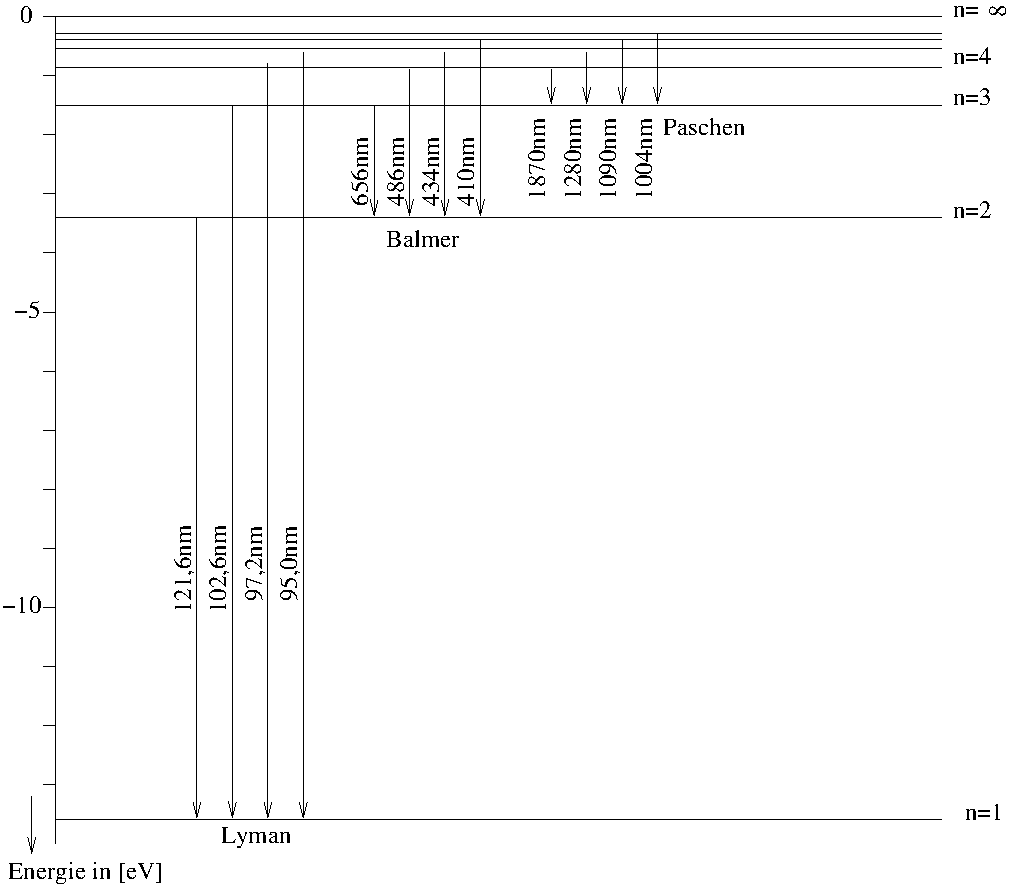
\includegraphics[scale=0.75]{waterstof}
\par\end{centering}

\caption{De energiebanen voor een elektron in waterstof}
\end{figure}



\paragraph*{Opdracht 3:}

\emph{Leg uit hoe het komt dat de atoomsoort aan het geabsorbeerde
of ge�miteerde licht te herkennen is.}


\section{Absorptielijnen}

Als twee ladingen in de vrije ruimte oneindig ver van elkaar af zijn,
ondervinden ze geen kracht. Omdat deze bewering voor iedere lading
geldt, stellen we dat de elektrische energie deze twee ladingen dan
0eV is. De elektrische energie ligt hiermee eenduidig vast. Als de
ladingen naar elkaar bewegen zal er een kracht ontstaan. Verder wordt
er een weg door de lading afgelegd. Zoals bekend is, kunnen we nu
zeggen dat:

\begin{equation}
\triangle W=\mathbf{F}\triangle\boldsymbol{\mathbf{s}}
\end{equation}


Volgens formule 3.1 is de kracht als functie van de afstand te schrijven.
Hiermee is de verandering van de arbeid te berekenen:

\begin{equation}
\triangle W=\frac{q_{1}q_{2}}{4\pi\epsilon_{o}r^{2}}\triangle s*cos(\alpha)
\end{equation}


Als de kracht en de weg parallel zijn, geldt:

\begin{equation}
\triangle W=\frac{q_{1}q_{2}}{4\pi\epsilon_{o}r^{2}}\triangle r
\end{equation}


De arbeid is nu te vinden met:

\begin{equation}
W=\int\frac{q_{1}q_{2}}{4\pi\epsilon_{o}}\frac{1}{r^{2}}dr\Leftrightarrow W=\frac{q_{1}q_{2}}{4\pi\epsilon_{o}}\int\frac{1}{r^{2}}dr
\end{equation}


\begin{equation}
W_{begin\rightarrow eind}=\frac{q_{1}q_{2}}{4\pi\epsilon_{o}}(\frac{1}{r_{begin}}-\frac{1}{r_{eind}})
\end{equation}


Met formule \ref{eq:db7} weten we welke stralen zijn toegestaan:

\begin{equation}
W_{begin\rightarrow eind}=\frac{q_{1}q_{2}}{4\pi\epsilon_{o}}(\frac{\pi mq_{1}q_{2}}{\epsilon_{0}n_{1}^{2}h^{2}}-\frac{\pi mq_{1}q_{2}}{\epsilon_{0}n_{2}^{2}h^{2}})
\end{equation}


\begin{equation}
W_{begin\rightarrow eind}=\frac{mq_{1}^{2}q_{2}^{2}}{4\epsilon_{0}^{2}h^{2}}(\frac{1}{n_{1}^{2}}-\frac{1}{n_{2}^{2}})
\end{equation}


Een deel van de elektrische energie wordt omgezet in kinetische energie.
Omdat de snelheid van het elektron rond een atoom veel lager dan de
lichtsnelheid is, geldt bij benadering:

\begin{equation}
E_{kin}=\frac{1}{2}mv^{2}=\frac{1}{2}\frac{p^{2}}{m}=\frac{1}{2}\frac{q_{1}q_{2}}{4\pi\epsilon_{0}r}=\frac{1}{2}\frac{q_{1}q_{2}}{4\pi\epsilon_{0}}\frac{\pi mq_{1}q_{2}}{\epsilon_{0}n^{2}h^{2}}=\frac{mq_{1}^{2}q_{2}^{2}}{8\epsilon_{0}^{2}h^{2}}(\frac{1}{n_{1}^{2}}-\frac{1}{n_{2}^{2}})
\end{equation}


Bij een elektronverval wordt de elektrische energie gebruikt voor
het versnellen van het elektron en voor het vrijkomen van een foton.
\begin{equation}
W_{begin\rightarrow eind}=E_{kin}+E_{foton}\Longleftrightarrow E_{foton}=W_{begin\rightarrow eind}-E_{kin}
\end{equation}
-

\begin{equation}
E_{foton}=\frac{mq_{1}^{2}q_{2}^{2}}{8\epsilon_{0}^{2}h^{2}}(\frac{1}{n_{1}^{2}}-\frac{1}{n_{2}^{2}})
\end{equation}


\begin{equation}
h\upsilon=h\frac{c}{\lambda}=\frac{mq_{1}^{2}q_{2}^{2}}{8\epsilon_{0}^{2}h^{2}}(\frac{1}{n_{1}^{2}}-\frac{1}{n_{2}^{2}})
\end{equation}


\begin{equation}
\frac{1}{\lambda}=\frac{mq_{1}^{2}q_{2}^{2}}{8\epsilon_{0}^{2}ch^{3}}(\frac{1}{n_{1}^{2}}-\frac{1}{n_{2}^{2}})=R(\frac{1}{n_{1}^{2}}-\frac{1}{n_{2}^{2}})\label{eq:rydberg}
\end{equation}


Hierin is $R$ de Rydberg constante. Met formule \ref{eq:rydberg}
is de golflengte van een ge�mitteerd foton te bepalen. Als een foton
wordt geabsorbeerd neemt het elektron energie op door naar een hogere
baan te gaan. Het atoom komt in een aangeslagen toestand.
\end{document}
